\subsection{Circuito per le misure in coincidenza}

Per misurare soltanto l'energia dei fotoni che hanno subito diffusione Compton, realizziamo una coincidenza temporale tra i due PMT. Sappiamo che il PMT1 deve avere un'alimentazione inferiore ai \SI{1800}V; facendo varie prove notiamo che il rate di coincidenze tra \SI{1500}V e \SI{1800}V rimane circa invariato. Impostiamo allora la tensione di alimentazione del PMT1 a \SI{1700}V in modo da avere un'alta efficienza ed essere lontani da zone in cui il dispositivo è malfunzionante.
\marginpar{Ho letto dal logbook che questo lo abbiamo fatto dopo, ma penso che mentire a favore del filo logico non ci nuocia in questo caso.\\
Forse dobbiamo parlare dei pocci con l'attenuatore  e dei retrigger.}

Il circuito di misura è stato poi ottimizzato e segue lo schema di \autoref{sc_conc}. Il segnale positivo del PMT2 è rimasto collegato al formatore come nelle misure precedenti (\autoref{???}) e la sua uscita negativa, invece di essere usata come trigger dell'ADC, viene inviata, dopo le opportune precauzioni di antiretrigger, ad un modulo di coincidenze%
\footnote{Stiamo sottintendendo che i conteggi dei PMT ed il numero di coincidenze siano mostrati dal contatore. Anche loro vengono da cavi che hanno superato il circuito di antiretrigger.}.

Il segnale del PMT1  viene ritardato di \SI{22}{ns} per essere messo in tempo con il discriminatore dell'altro PMT. Esso è poi collegato al discriminatore che poi va al \texttt{gate \& delay} che funge da antiretrigger.
\marginpar{in realtà ci sono stati lo stesso degli antiretrigger ma molto meno del poccio che fanno i discriminatori}

L'uscita del modulo di coincidenza è poi portata ad un modulo \texttt{gate \& delay} che la ritarda e la allunga per avere un segnale di trigger con le stesse caratteristiche della sezione precedente.

%%%%%%%%%%%%%%%%%%%%%%%%%%%%%%%%%%%%%%%%%%%%%%%%%%%%%%%%%%%%%%%

\subsection{Caratteristiche geometriche del fascio}

\subsubsection{Accorgimenti sperimentali}

Ci interessa misurare la divergenza angolare del fascio di cui terremo conto nel Monte Carlo in \autoref{simulazione}.
\marginpar{mettere il label nella sezione opportuna}
Per farlo posizioniamo il PMT2 di fronte alla sorgente a vari angoli e triggeriamo sul PMT2 stesso. Lo scopo è disegnare un grafico dei rate in funzione dell'angolo.

Per fare questa misura colleghiamo una \texttt{time unit} che faremo partire a mano azionando la levetta \emph{start} e la bloccheremo spostando la levetta sulla posizione \emph{reset}. Impostando la manopola della durata temporale sulla posizione ``$\infty$'' abbiamo un segnale \texttt{NIM} costantemente a livello 1. Collegando l'uscita della \texttt{time unit} all'ingresso \emph{start} del contatore possiamo farlo partire quando vogliamo e possiamo fermare il contatore collegando l'\emph{end marker} all'ingresso \emph{stop} di quest'ultimo. 
L'utilità di questo circuito sta nel fatto che, collegando un'altra uscita della \texttt{time unit} al modulo di coincidenze, è possibile attivare e disattivare il trigger dell'ADC ed il contatore contemporaneamente.

Per misurare meglio gli angoli abbiamo stampato un goniometro che abbiamo posizionato sotto la guida su cui scorre il PMT2 e lo abbiamo ritagliato in modo che il centro dell'immagine corrisponda al perno di rotazione di tale guida. Infine abbiamo tracciato un segmento sulla parte trasparente che ci permette di capire a quale angolo posizioniamo il PMT.

\subsubsection{Analisi dei dati e risultati}

\marginpar{lascio a Jack l'onore di scrivere tutto quello che ha fatto (Andrea)}

\begin{table}
\centering

\begin{tabular}{|c|c|}
\hline
angolo [\si{\degree}] & rate [\si{s^{-1}}] \\
\hline
$ 0 $ & $ 3788\pm11 $ \\ 

$ 1 $ & $ 3422\pm10 $ \\ 
$ 2 $ & $ 2690 \pm 9 $ \\ 
$ 3 $ & $ 1926 \pm 8 $ \\ 
$ 4 $ & $ 1156 \pm 6 $ \\ 

$ -1 $ & $ 3517\pm11 $ \\ 
$ -2 $ & $ 2843 \pm 9 $ \\ 
$ -3 $ & $ 2087 \pm 8 $ \\ 
$ -4 $ & $ 1306 \pm 6 $ \\ 
\hline
\end{tabular}

\caption{Dati considerati nel fit per determinare la forma del fascio. L'errore sugli angoli è 0.1$^{\circ}$.}
\label{tabfo}
\end{table}

\begin{figure}
\centering
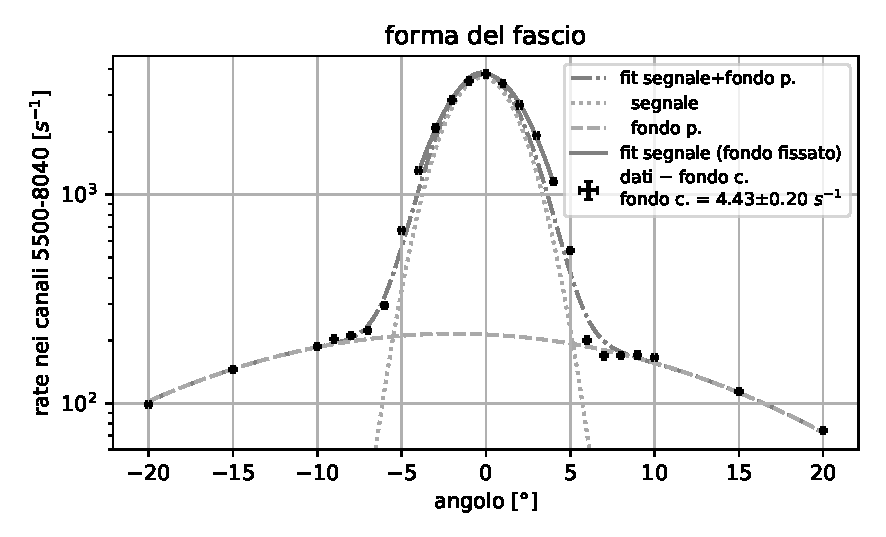
\includegraphics[width=25 em]{forma}
\caption{Fit della forma del fascio e relativo fondo.}
\label{forma}
\end{figure}



